%=====================================================
\section{Hasse Diagrams}
%=====================================================

\begin{frame}{Hasse Diagram}

\textbf{Definition}

A \textbf{Hasse Diagram} is a graphical representation of a partially
ordered set (poset), obtained by removing self-loops, arrowheads and
transitive edges.

\vspace{0.8cm}

\begin{block}{Purpose}

\vspace{0.1cm}
 It provides a simplified visualization of the ordering relationship between the elements of a poset.
\end{block}

\end{frame}

%=====================================================

\begin{frame}{Hasse Diagram of $\left(\mathcal P(A),\subseteq\right)$}

Let
\[
A=\{1,2\}
\]
Then
\[
\mathcal P(A)=
\left\{
\emptyset,\,
\{1\},\,
\{2\},\,
\{1,2\}
\right\}
\]
with the partial order
\[
R=\subseteq .
\]

\begin{columns}

\column{0.45\textwidth}

\centering

\begin{tikzpicture}[scale=1.1]

\node (e) at (0,0) {$\emptyset$};

\node (1) at (-1.2,1.5) {$\{1\}$};
\node (2) at (1.2,1.5) {$\{2\}$};

\node (12) at (0,3) {$\{1,2\}$};

\draw (e)--(1);
\draw (e)--(2);
\draw (1)--(12);
\draw (2)--(12);

\end{tikzpicture}

\column{0.55\textwidth}

\textbf{Observation}

\begin{itemize}
\item $\emptyset$ is the least element.
\item $\{1,2\}$ is the greatest element.
\item $\{1\}$ and $\{2\}$ are incomparable.
\item This is a partially ordered set.
\end{itemize}

\end{columns}

\end{frame}

%=====================================================
\begin{frame}{Hasse Diagram of $\left(\mathcal P(A),\subseteq\right)$}
\[Let\;
A=\{1,2,3\},
S=\mathcal P(A),
R=\subseteq.
\; Then,\;
(S,R)
\; is\; a\; partially\;ordered\;set\]
\centering

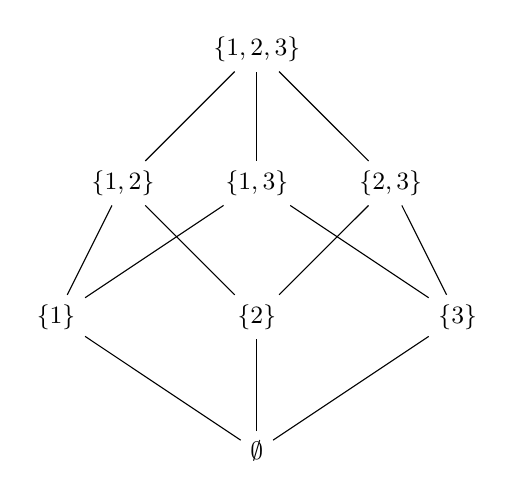
\begin{tikzpicture}[
    scale=0.85,
    every node/.style={font=\small}
]

% Bottom
\node (e) at (0,0) {$\emptyset$};

% Level 1
\node (1) at (-3,2) {$\{1\}$};
\node (2) at (0,2) {$\{2\}$};
\node (3) at (3,2) {$\{3\}$};

% Level 2
\node (12) at (-2,4) {$\{1,2\}$};
\node (13) at (0,4) {$\{1,3\}$};
\node (23) at (2,4) {$\{2,3\}$};

% Top
\node (123) at (0,6) {$\{1,2,3\}$};

% Edges
\draw (e)--(1);
\draw (e)--(2);
\draw (e)--(3);

\draw (1)--(12);
\draw (1)--(13);

\draw (2)--(12);
\draw (2)--(23);

\draw (3)--(13);
\draw (3)--(23);

\draw (12)--(123);
\draw (13)--(123);
\draw (23)--(123);

\end{tikzpicture}

\end{frame}